\pagebreak
\section{Auswertung}
\label{sec:Auswertung}

\subsection{A-Scan}
Aus den gemessenen Zeiten können über \eqref{eqn} die Tiefen $d_{1/2}$ ausgerechnet werden. Es wird eine Laufzeitkorrektur von
\begin{equation}
  t_\text{korr} = \SI{0.5}{µs},
\end{equation}
bedingt durch die Schutzschicht auf der Ultraschallsonde, abgezogen. Der Durchmesser der Störstellen $2r$ wird über
\begin{equation}
  2r = h - d_1 - d_2
\end{equation} mit der gemessenen Höhe
\begin{equation}
  h = \SI{80.04}{mm}
\end{equation}
des Acrylblocks berechnet. Dabei wird eine Schallgeschwindigkeit in Acryl von $\SI{2730}{\meter\per\second}$ \cite{olympus} angenommen. Die Ergebnisse, sowie die mit dem Messschieber gemessenen Längen finden sich in Tab.~\ref{tab:a}.
\begin{table}
        \caption{Messergebnisse aus dem A-Scan. Neben den abgelesenen und berechneten Daten $d_n$ sind auch die zuvor mittels Messschieber bestimmten Abmessungen $d_n^\text{mech}$ eingetragen.}
        \centering
        \label{tab:a}
        \begin{tabular}{l@{}S[round-mode=off, table-format=2.0]S[table-format=2.3, round-precision=4, round-mode=off] S[table-format=2.2, round-precision=4, round-mode=figures] S[table-format=1.4, round-precision=4, round-mode=figures] S[table-format=2.3, round-precision=4, round-mode=figures] S[table-format=2.2, round-precision=4, round-mode=figures] S[table-format=2.4, round-precision=4, round-mode=off] } \toprule & {$\text{Störstelle}$}& {$d_1/\si{mm}$}& {$d_2/\si{mm}$}& {$2r/\si{mm}$}& {$d_1^\text{mech}/\si{mm}$}& {$d_2^\text{mech}/\si{mm}$}& {$2r^\text{mech}/\si{mm}$}\\\midrule
& 1 & 18.02 & 61.56149999999999522515 & 0.46050000000000257394 & 19.62000000000000099476 & 59.61999999999999744205 & 0.80 \\
& 2 & 19.93 & 59.78699999999999192823 & 0.32400000000000828138 & 17.76000000000000156319 & 61.29999999999999715783 & 0.98 \\
& 3 & 61.29 & 13.78650000000000019895 & 4.96500000000000429878 & 61.28000000000000113687 & 13.43999999999999950262 & 5.32 \\
& 4 & 54.05 & 22.11299999999999599254 & 3.87300000000000821387 & 53.84000000000000341061 & 21.69999999999999928946 & 4.50 \\
& 5 & 46.68 & 30.43950000000000244427 & 2.91749999999998976818 & 46.50000000000000000000 & 30.07999999999999829470 & 3.46 \\
& 6 & 39.04 & 39.03900000000000147793 & 1.96199999999999152855 & 38.60000000000000142109 & 38.71999999999999886313 & 2.72 \\
& 7 & 31.12 & 47.09249999999999403144 & 1.82550000000000767209 & 30.82000000000000028422 & 46.88000000000000255795 & 2.34 \\
& 8 & 23.07 & 55.14600000000000079581 & 1.82550000000000411937 & 22.78000000000000113687 & 54.82000000000000028422 & 2.44 \\
& 9 & 15.01 & 62.92650000000001142553 & 2.09849999999999115019 & 14.82000000000000028422 & 62.97999999999999687361 & 2.24 \\
& 10 & 7.23 & 70.98000000000000397904 & 1.82549999999999990052 & 6.87999999999999989342 & 70.79999999999999715783 & 2.36 \\
& 11 & 55.82 & 15.42450000000000009948 & 8.78699999999999548095 & 55.11999999999999744205 & 14.63000000000000078160 & 10.29 \\
 \bottomrule \end{tabular} \end{table}


\subsection{B-Scan}
Die gleiche Messung wird erneut mit einem B-Scan durchgeführt und wie zuvor ausgewertet. Hier wurde keine Laufzeitkorrektur durchgeführt, da die Werte bereits ohne diese gut zu den mechanisch ermittelten Längen passen. Die grafischen Darstellungen der Scans finden sich in Abb.~\ref{fig:b1} und~\ref{fig:b2}. Daraus werden die in Tab.~\ref{tab:b} notierten Längen bestimmt.
\fig{build/b1.pdf}{Grafische Darstellung des ersten B-Scans (von oben), sowie der bestimmten Längen.}{b1}
\fig{build/b2.pdf}{Grafische Darstellung des zweiten B-Scans (von unten), sowie der bestimmten Längen. Störstelle 10 war in einer anderen Farbtabelle ablesbar (siehe Abb.~\ref{fig:b3} im Anhang), die jedoch viel Rauschen erzeugte. Daher wurde die hier vorliegende Farbtabelle benutzt und nur der Messwert eingetragen.}{b2}
\FloatBarrier
\begin{table}
        \caption{Messergebnisse aus dem B-Scan.}
        \centering
        \label{tab:b}
        \begin{tabular}{l@{}S[round-mode=off, table-format=2.0]S[table-format=2.3, round-precision=2, round-mode=places] S[table-format=2.2, round-precision=4, round-mode=figures] S[table-format=1.4, round-precision=4, round-mode=figures] S[table-format=2.3, round-precision=4, round-mode=figures] S[table-format=2.2, round-precision=4, round-mode=figures] S[table-format=2.4, round-precision=2, round-mode=places] } \toprule & {$\text{Störstelle}$}& {$d_1/\si{mm}$}& {$d_2/\si{mm}$}& {$2r/\si{mm}$}& {$d_1^\text{mech}/\si{mm}$}& {$d_2^\text{mech}/\si{mm}$}& {$2r^\text{mech}/\si{mm}$}\\\midrule& 1 & 19.79250000000000042633 & 60.05999999999999516831 & 0.18750000000000016653 & 19.62000000000000099476 & 59.61999999999999744205 & 0.80000000000000426326 \\
& 2 & 17.74500000000000099476 & 61.42499999999999005240 & 0.87000000000000965450 & 17.76000000000000156319 & 61.29999999999999715783 & 0.98000000000000397904 \\
& 3 & 61.42499999999999005240 & 13.64999999999999857891 & 4.96500000000000785150 & 61.28000000000000113687 & 13.43999999999999950262 & 5.32000000000000561329 \\
& 4 & 53.91749999999999687361 & 21.83999999999999985789 & 4.28250000000000152767 & 53.84000000000000341061 & 21.69999999999999928946 & 4.50000000000000355271 \\
& 5 & 46.40999999999999658939 & 30.02999999999999758415 & 3.60000000000000230926 & 46.50000000000000000000 & 30.07999999999999829470 & 3.46000000000000795808 \\
& 6 & 39.31199999999999761258 & 38.90249999999999630518 & 1.82550000000000078870 & 38.60000000000000142109 & 38.71999999999999886313 & 2.72000000000000596856 \\
& 7 & 30.71249999999999502620 & 47.09249999999999403144 & 2.23500000000000786926 & 30.82000000000000028422 & 46.88000000000000255795 & 2.34000000000000341061 \\
& 8 & 23.47799999999999798206 & 54.59999999999999431566 & 1.96200000000000551736 & 22.78000000000000113687 & 54.82000000000000028422 & 2.44000000000000483169 \\
& 9 & 15.01499999999999879208 & 62.78999999999999914735 & 2.23500000000000076383 & 14.82000000000000028422 & 62.97999999999999687361 & 2.24000000000000198952 \\
& 10 & 7.09799999999999986500 & 71.66249999999999431566 & 1.27950000000001673506 & 6.87999999999999989342 & 70.79999999999999715783 & 2.36000000000001364242 \\
& 11 & 55.96500000000000341061 & 15.01499999999999879208 & 9.06000000000000049738 & 55.11999999999999744205 & 14.63000000000000078160 & 10.29000000000000802913 \\
 \bottomrule \end{tabular} \end{table}


\subsection{TM-Scan}
Zuletzt wird das Herzmodell, beschrieben in Abschnitt~\ref{sec:durchführung}, untersucht. Der TM-Scan ist in Abb.~\ref{fig:tm1} und~\ref{fig:tm2} zu finden. Die Herzfrequenz ist
\begin{equation}
  \nu_\text{Herz} = \frac{16}{\SI{25}{s}} = \SI{0.64}{\hertz} = \SI{38.4}{\per\minute}.
\end{equation}
Für die Schallgeschwindigkeit in Wasser wird hier
\begin{equation}
  c = \SI{1480}{\meter\per\second},
\end{equation}
ebenfalls aus \cite{olympus}, angenommen.
Es ergibt sich
\begin{align*}
  \Delta t_\text{A-Scan} &= \SI{48.4}{µs} - \SI{16.2}{µs} \\
  \Delta t_\text{TM-Scan} &= \SI{44}{µs} - \SI{3}{µs} \\
  \Delta d_\text{A-Scan} &= \SI{2.38}{cm} \\
  \Delta d_\text{TM-Scan} &= \SI{3.03}{cm}.
\end{align*}
Daraus folgt über das Volumen eines Kugelsegments (\cite{wurst}) das Schlagvolumen
\begin{equation}
  SV = \frac{1}{3} \pi (\Delta d)^2 (3R - \Delta d)
\end{equation}
als Schlagvolumen
\begin{align*}
  SV_\text{A-Scan} &= \SI{67.17}{\cubic\centi\meter} \\
  SV_\text{TM-Scan} &= \SI{102.62}{\cubic\centi\meter}
\end{align*}
und über
\begin{equation}
  HZV = SV \cdot \nu_\text{Herz}
\end{equation}
das Herzzeitvolumen
\begin{align*}
  HZV_\text{A-Scan} &= \SI{42.99}{\cubic\centi\meter\per\second} \\
  HZV_\text{TM-Scan} &= \SI{65.68}{\cubic\centi\meter\per\second}.
\end{align*}

\fig{build/tm.pdf}{Time-Motion-Scan des Herzmodells.}{tm1}
\fig{build/tm_zoom.pdf}{Kleinerer Zeitausschnitt aus dem Time-Motion-Scan.}{tm2}
\FloatBarrier
\subsection{Messdaten}
\input{build/a_d.tex}

\fig{build/b3.pdf}{Variante von Abb.~\ref{fig:b2} mit veränderter Farbtabelle, Störstelle 10 ist deutlich zu erkennen.}{b3}
\begin{figure}
  \centering
  \begin{subfigure}{0.48\textwidth}
    \centering
    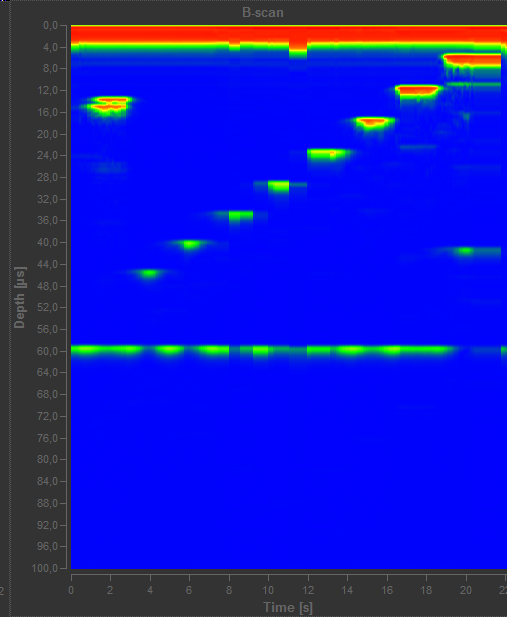
\includegraphics[width=\textwidth]{daten/b/1.png}
    \caption{Erster Scan, von oben.}
    \label{fig:db1}
  \end{subfigure}
  \begin{subfigure}{0.48\textwidth}
    \centering
    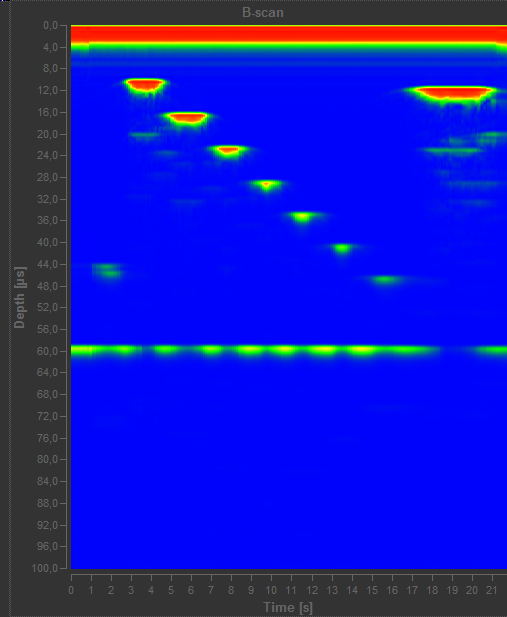
\includegraphics[width=\textwidth]{daten/b/2.png}
    \caption{Zweiter Scan, von unten.}
    \label{fig:db2}
  \end{subfigure}
  \caption{Originalbilder der B-Scans.}
  \label{fig:db}
\end{figure}
\fig{daten/tm/scan.png}{Originalbild des TM-Scans.}{dtm}[width=0.5\textwidth]
